En este capítulo se tratará la propuesta de solución seleccionada en el capítulo anterior. Se tratarán los objetivos fijando uno general y varios específicos, así como los requerimientos que necesita el sistema pero que nuestros usuarios no verán de manera directa. El modelo de despliegue del sistema, que muetsra de manera gráfica como se planea interconectar nuestro sistema dentro de la empresa, y las especificaciones de plataforma, que son los requisitos que requiere el equipo que se planea usar para hacer funcionar el sistema.

%--------------------------------------------------
\section{Objetivos}

% - - - - - - - - - - - - - - - - - - - - - - - - -
\subsection{Objetivo general}

Desarrollar un sistema de software que facilite y optimice los procesos de administraci\'on de citas, consulta de expedientes y administraci\'on de la farmacia de una cl\'inica mediana.

% - - - - - - - - - - - - - - - - - - - - - - - - -
\subsection{Objetivos específicos}

- Reducir el tiempo para registrar una cita.

- Permitir el registro de citas a través de internet.

- Facilitar la gestión, cambio y cancelación y de citas.

- Facilitarle a los pacientes y a los médicos la consulta de expedientes clínicos

- Evitar el deterioro de los expedientes clínicos.

- Facilitar y agilizar la consulta de medicamentos disponibles en la farmacia.

- Mantener un control preciso de los ingresos obtenidos en el consultorio, así como del inventario.

- Facilitar la creación de recetas y asegurar su legibilidad.

%--------------------------------------------------
\section{Modelo de despliegue}


% - - - - - - - - - - - - - - - - - - - - - - - - -
\subsection{Requerimientos no funcionales}

ID: RNF 1.

Nombre: Cumplimiento de la Ley Federal de Protección de Datos Personales en posesión de los particulares.

Descripción: El sistema cumplirá esta ley con los datos de los pacientes que se encuentren almacenados en el expediente. \\

ID: RNF 2.

Nombre: Seguimiento del Manual del Expediente Clínico Electrónico (SALUD).

Descripción: El sistema manejará el manual del expediente clínico médico para registrar los expedientes, extrayendo los datos más importantes de dicho manual para solucionar el problema. \\

ID: RNF 3.

Nombre: Cumplimiento de la Norma Oficial Mexicana NOM-004-SSA3-2012.

Descripción: El expediente médico cumplirá dicha norma para su generación y almacenamiento. \\

ID: RNF 4.

Nombre: Confidencialidad en el manejo de datos de un paciente.

Descripción: El sistema no permitirá el acceso a otras personas que no sean las autorizadas para ver o editar los datos de un paciente. \\

ID: RNF 5. 

Nombre: Plataforma web para el manejo de forma instintiva.

Descripción: La plataforma de generación de citas se desarrollará de forma web para que su uso sea más sencillo. \\

ID: RNF 6.

Nombre: Disponibilidad del sitio web para la generación de citas.

Descripción: El sitio web donde se podrá solicitar una cita estará disponible las 24 horas del día.

% - - - - - - - - - - - - - - - - - - - - - - - - -
\subsection{Modelo de despliegue del sistema}

Diagrama de despliegue presentando los sistemas (comunicaciones, sistemas externos y software de base) con los que interactúa el sistema y su explicación. vea los siguientes cuatro ejemplos.

	\begin{figure}[htbp!]
		\centering
			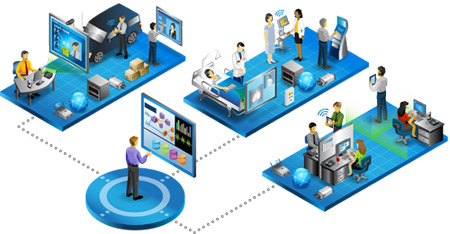
\includegraphics[width=0.8\textwidth]{images/arquitectura1}
		\caption{Diagrama de arquitectura.}
	\end{figure}

	\begin{figure}[htbp!]
		\centering
			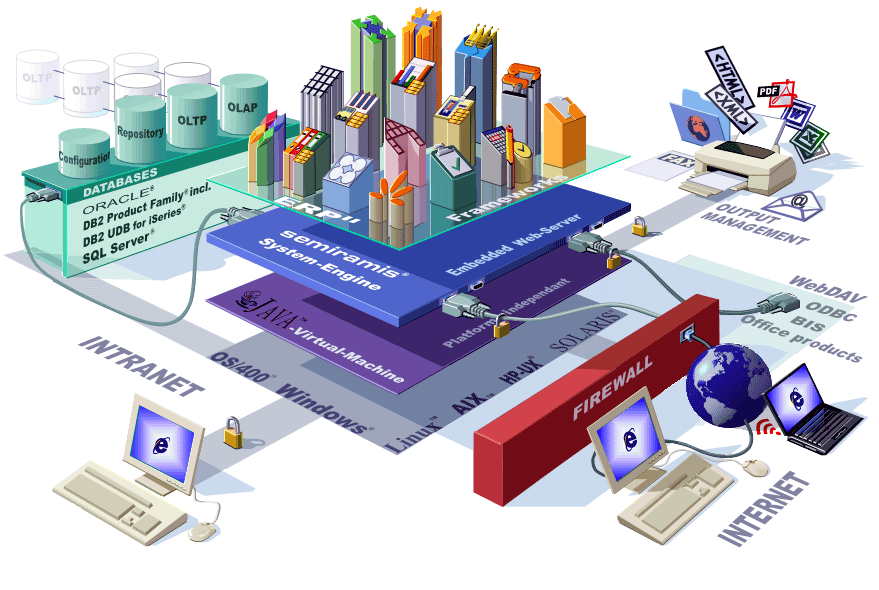
\includegraphics[width=0.8\textwidth]{images/arquitectura2}
		\caption{Diagrama de arquitectura.}
	\end{figure}

	\begin{figure}[htbp!]
		\centering
			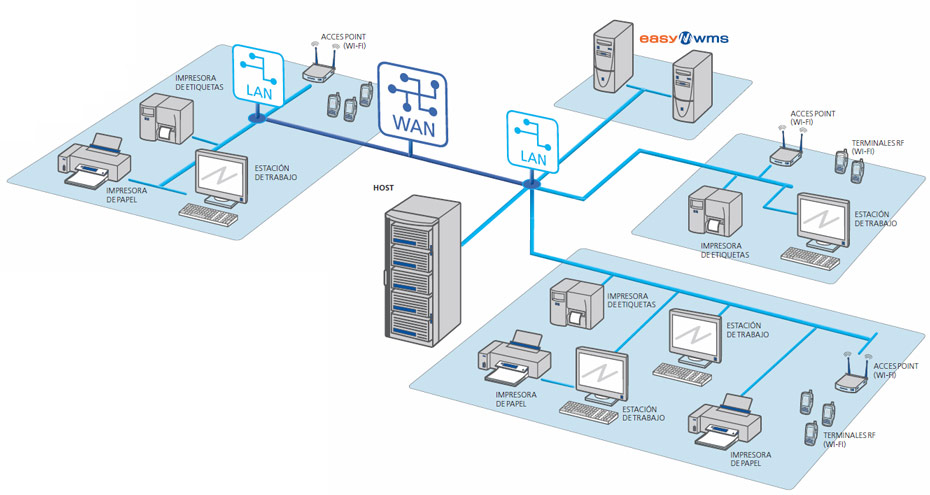
\includegraphics[width=0.8\textwidth]{images/arquitectura3}
		\caption{Diagrama de arquitectura.}
	\end{figure}

	\begin{figure}[htbp!]
		\centering
			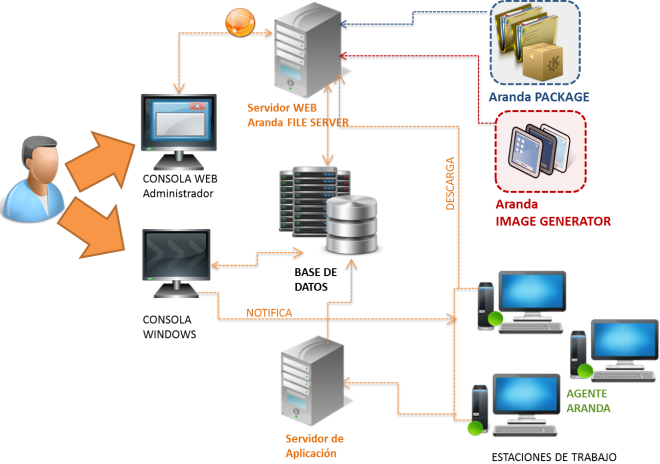
\includegraphics[width=0.8\textwidth]{images/arquitectura4}
		\caption{Diagrama de arquitectura.}
	\end{figure}


% - - - - - - - - - - - - - - - - - - - - - - - - -
\subsection{Especificación de Plataforma}

Hardware requerido:

- Computadora con procesador de al menos 1 GHz, con 1 GB de memoria RAM. \\

Software requerido:

- Java.

- Navegador web. \\

Servicios requeridos:

- Internet. \\

